\chapter{Making MATSim Agents Smarter with the Belief-Desire-Intention Framework}
\label{ch:bdi}
% ##################################################################################################################

\hfill \textbf{Authors:} Lin Padgham, Dhirendra Singh

\begin{center} 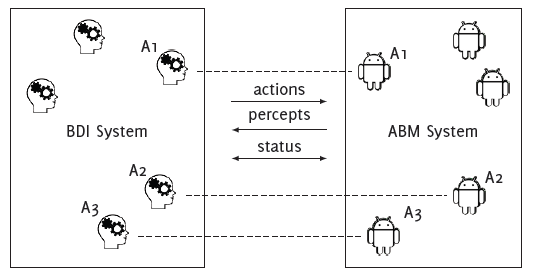
\includegraphics[width=0.65\textwidth, angle=0]{extending/figures/bdi/title.png} \end{center}

\createStandardInformation{bdiintegration}{\lstinline|RunBDIWithinDayExample| class}{bdiintegration}{\citet{ecai}}

% ##################################################################################################################
\section{Introduction}
\label{sec:bdi-intro}
In this chapter we introduce an extension to \gls{matsim} that allows a
developer to program (some of) the decision making of an agent in a \gls{bdi} system, while the actual actions, and
perception of the environment happen within \gls{matsim}. This allows for
sophisticated modeling of human-like agents, within a \gls{bdi}
framework, using the concepts of goals, hierarchical abstract plans,
which contain sub-goals, and percepts which are information from the
environment, as well as beliefs about the current situation. For
example we have used it to model residents in a 
bushfire evacuation as well as an incident controller in an evacuation
scenario. The residents may receive percepts about the bushfire from
the fire simulation as well as warnings and messages from the incident
controller agent. They may
have goals to pick up children, check on neighbors, communicate with
other family members etc. Their plans will result in
decision making which at various points includes actions which are then
executed within \gls{matsim}.

In the standard usage of \gls{matsim} the intelligence in the behavior of
the individual agents arises from the  co-evolutionary algorithms in
the replanning phase. This is based on agents evaluating via a scoring
function, the plan they have executed during a given day, and
modifying this to obtain a new plan until all agents have sufficiently good
plans and the system reaches a stable state. This approach however
does not work for applications where one cannot assume that the agents
adjust and refine their behavior over many iterations, to eventually
obtain their standard modus operandi. For applications such as
emergency management, agents must react immediately to the situation
as it evolves, doing so in an ``intelligent'' manner. 

The chapter on Within-Day Replanning introduces two approaches to the
\gls{mobsim} component which address the need to be more reactive to the
evolving situation. The first allows a centralized \gls{matsim} process to
identify sets of agents that should have their plans modified, then
runs one or more processes to adjust the plans of these agents. The
second takes the approach of rewriting the agent so that instead of
following a specified plan, the agent invokes a decision making
process at all possible decision points. By integrating a \gls{bdi} agent
platform with \gls{matsim} \citep{ecai} we allow autonomous individual
decision making to be programmed in specialized and powerful systems
that have been developed specifically for this purpose, balancing
reactive behavior and goal based commitment. Different \gls{bdi} platforms
have different strengths but are in general based on a simplified
psychological/philosophical view of how people behave, facilitating a
high level specification of complex human behavior. These systems have
been demonstrated to be very efficient for building complex
applications \citep{benfield}.  Providing the appropriate system
interface support is developed, any \gls{bdi} system can be coupled to
\gls{matsim} as described here. We have currently used three different \gls{bdi}
systems, for which the system level interface is available.  The
decisions made in the \gls{bdi} system are then inserted into the \gls{matsim}
plans of the relevant agents, allowing the \gls{matsim} agents to operate in
the same efficient manner as in standard \gls{matsim}.

% ##################################################################################################################
\section{Software Structure}
\label{sec:bdi-structure}
Our framework supports the independent execution of \gls{matsim} and the \gls{bdi} platform, with 
synchronization via the infrastructure provided.
They can either run within a single process (in
separate synchronized threads or in a single thread sequentially), or in two
separate processes (synchronizing using inter-process communication, such as
sockets). The former is of course considerably more efficient. 
%
Conceptually, for every \gls{matsim} agent whose decision making is to be
done in the \gls{bdi} system, a \gls{bdi} agent must be created. The \gls{bdi} counterpart can
be regarded as ``the brain'' associated with the \gls{matsim} agent. It is
possible to have \gls{bdi} agents with no \gls{matsim} counterpart and vice
versa. For example, in our bushfire application, the incident
controller has no \gls{matsim} agent, as he does not move on the road
network. He receives information about the fire, and has some static
location information, and his role in the simulation is to issue
warnings and evacuation advisories, which in turn affects the resident
agents. There may also be \gls{matsim} agents that do not have a \gls{bdi}
counterpart. For example in a taxi modeling application, there may be
\gls{matsim} agents using the road network, but without any need for
modeling of complex decision making, and these may exist only within
\gls{matsim}. 

Figure~\ref{architecture} shows the basic architecture of the
two parallel systems and the information which is passed between them
at each timestep.

%\begin{figure}
%\centering
%\resizebox{0.75\textwidth}{!}{
%\begin{tikzpicture}
\tikzstyle{active}=[draw=red, fill=red!20, very thick, draw]

\node[above=1.1cm, xshift=2.75cm, label={[label distance=-0.3cm]120:A1}]
(bdi1) {
\includegraphics[height=0.8cm]{extending/figures/bdi/fig-braincogs.png}};

\node[below=0.45cm,xshift=2.5cm, label={[label distance=-0.3cm]120:A2}]
(bdi2) {
\includegraphics[height=0.8cm]{extending/figures/bdi/fig-braincogs.png}};

\node[below=1.3cm, xshift=1.5cm, label={[label distance=-0.3cm]120:A3}] 
(bdi3) {
\includegraphics[height=0.8cm]{extending/figures/bdi/fig-braincogs.png}};

\node[above=0.5cm]
(bdi4) {
\includegraphics[height=0.8cm]{extending/figures/bdi/fig-braincogs.png}};

\node[above=1.75cm, xshift=1cm]
(bdi5){
\includegraphics[height=0.8cm]{extending/figures/bdi/fig-braincogs.png}}; 


\node[above=1.1cm,xshift=7cm, label={[label distance=-0.3cm]30:A1}]
(abm1) {
\includegraphics[height=0.8cm]{extending/figures/bdi/fig-robot.png}};

\node[below=0.45cm, xshift=9cm, label={[label distance=-0.3cm]30:A2}] 
(abm2) {
\includegraphics[height=0.8cm]{extending/figures/bdi/fig-robot.png}}; 

\node[below=1.3cm, xshift=7.2cm, label={[label distance=-0.2cm]30:A3}]
(abm3) {
\includegraphics[height=0.8cm]{extending/figures/bdi/fig-robot.png}}; 

\node[above=1.75cm, xshift=9cm] 
(abm4) {
\includegraphics[height=0.8cm]{extending/figures/bdi/fig-robot.png}}; 

\node[above=0.75cm, xshift=9.5cm] 
(abm5) {
\includegraphics[height=0.8cm]{extending/figures/bdi/fig-robot.png}}; 
\draw[densely dashed](bdi1)--(abm1);
\draw[densely dashed](bdi2)--(abm2);
\draw[densely dashed](bdi3)--(abm3);
\begin{pgfonlayer}{background}
\node [fit=(bdi1) (bdi2) (bdi3) (bdi4) (bdi5)]
[rectangle, minimum height=4cm, minimum width=2.5cm, draw]{BDI System};
\node [fit=(abm1) (abm2) (abm3) (abm4) (abm5)]
[rectangle, minimum height=4cm, minimum width=2.5cm, draw]{ABM System};
\draw [->, >=latex,] (4,1.0) -- node[above]{actions} (6,1.0);
\draw [<-, >=latex,] (4,0.4) -- node[above]{percepts} (6,0.4);
\draw [<->, >=latex,] (4,-0.2) -- node[above]{status} (6,-0.2);
\end{pgfonlayer}
\end{tikzpicture}


%}
%\caption{Conceptual BDI-\gls{abms} integration architecture}
%\label{architecture}
%\end{figure} 

\createfigure%
{Conceptual BDI-\gls{abms} integration architecture}%
{Conceptual BDI-\gls{abms} integration architecture}%
{\label{architecture}}%
{\resizebox{0.75\textwidth}{!}{\begin{tikzpicture}
\tikzstyle{active}=[draw=red, fill=red!20, very thick, draw]

\node[above=1.1cm, xshift=2.75cm, label={[label distance=-0.3cm]120:A1}]
(bdi1) {
\includegraphics[height=0.8cm]{extending/figures/bdi/fig-braincogs.png}};

\node[below=0.45cm,xshift=2.5cm, label={[label distance=-0.3cm]120:A2}]
(bdi2) {
\includegraphics[height=0.8cm]{extending/figures/bdi/fig-braincogs.png}};

\node[below=1.3cm, xshift=1.5cm, label={[label distance=-0.3cm]120:A3}] 
(bdi3) {
\includegraphics[height=0.8cm]{extending/figures/bdi/fig-braincogs.png}};

\node[above=0.5cm]
(bdi4) {
\includegraphics[height=0.8cm]{extending/figures/bdi/fig-braincogs.png}};

\node[above=1.75cm, xshift=1cm]
(bdi5){
\includegraphics[height=0.8cm]{extending/figures/bdi/fig-braincogs.png}}; 


\node[above=1.1cm,xshift=7cm, label={[label distance=-0.3cm]30:A1}]
(abm1) {
\includegraphics[height=0.8cm]{extending/figures/bdi/fig-robot.png}};

\node[below=0.45cm, xshift=9cm, label={[label distance=-0.3cm]30:A2}] 
(abm2) {
\includegraphics[height=0.8cm]{extending/figures/bdi/fig-robot.png}}; 

\node[below=1.3cm, xshift=7.2cm, label={[label distance=-0.2cm]30:A3}]
(abm3) {
\includegraphics[height=0.8cm]{extending/figures/bdi/fig-robot.png}}; 

\node[above=1.75cm, xshift=9cm] 
(abm4) {
\includegraphics[height=0.8cm]{extending/figures/bdi/fig-robot.png}}; 

\node[above=0.75cm, xshift=9.5cm] 
(abm5) {
\includegraphics[height=0.8cm]{extending/figures/bdi/fig-robot.png}}; 
\draw[densely dashed](bdi1)--(abm1);
\draw[densely dashed](bdi2)--(abm2);
\draw[densely dashed](bdi3)--(abm3);
\begin{pgfonlayer}{background}
\node [fit=(bdi1) (bdi2) (bdi3) (bdi4) (bdi5)]
[rectangle, minimum height=4cm, minimum width=2.5cm, draw]{BDI System};
\node [fit=(abm1) (abm2) (abm3) (abm4) (abm5)]
[rectangle, minimum height=4cm, minimum width=2.5cm, draw]{ABM System};
\draw [->, >=latex,] (4,1.0) -- node[above]{actions} (6,1.0);
\draw [<-, >=latex,] (4,0.4) -- node[above]{percepts} (6,0.4);
\draw [<->, >=latex,] (4,-0.2) -- node[above]{status} (6,-0.2);
\end{pgfonlayer}
\end{tikzpicture}

}}%
{}

The structure of the data components passed between the \gls{matsim} agent
and its \gls{bdi} counterpart is shown in Table~\ref{interfacedata} and
consists of {\it BDI Actions}\footnote{We call these actions \gls{bdi}
  Actions to distinguish them from actions in the \gls{abms} which may
  include lower level or additional actions.}, {\it Percepts} and {\it
  Queries}. As indicated in Figure~\ref{architecture} \gls{bdi}-actions are
always initiated by the \gls{bdi} system. Their status field however can be
modified by both systems.  When a \gls{bdi} action such as
\lstinline{DriveTo(loc)} is decided by the \gls{bdi} agent, the \gls{bdi} system
sets the status of this action to be ``INITIATED''. \gls{matsim} will then
set its status to ``RUNNING'' which will likely stay in this state for
some number of steps. When the \lstinline{loc} destination is reached
the \gls{matsim} routine will set the status to ``PASSED'' and the \gls{bdi}
system will continue reasoning about the next piece of agent
behaviour. If desired, the \gls{matsim} routine can also detect situations
which should be conveyed as ``FAILED'' and pass this to the \gls{bdi}
counterpart. For example if there is a \gls{bdi} action to meet at a
location and time, and the \gls{matsim} agent is delayed in traffic, the \gls{bdi}
action implementation in \gls{matsim} can be programmed to detect the
passing of the deadline and set the status to ``FAILED'' at which
point the \gls{bdi} agent will attempt failure recovery (as part of the \gls{bdi}
infrastructure). The \gls{bdi} system can also set the status to 
``ABORTED''---for example if some information arrives, requiring a different
action---in which case it is canceled within \gls{matsim}. The \gls{bdi} system
can also set status to ``SUSPENDED'' though this is not currently
implemented.

\Omit{
 Our \gls{matsim} infrastructure will initially set
the status of an ``INITIATED'' action to be ``RUNNING'', and when it
completes it will be set to ``PASSED''.  It can also be set to ``FAILED''
by \gls{matsim}, based on an application specific assessment relevant to the
logic of the \gls{bdi}-action. The \gls{bdi} system can set the status to ``ABORTED'' and
potentially ``SUSPENDED'', which will cause \gls{matsim} to cease executing
the relevant \gls{bdi}-action either permanently or temporarily.
}

\begin{table}[h]
Components of the data package provided to specific agents via the
interface:\\ 
\begin{tabular}{ @{}p{0.15\textwidth} | p{0.8\textwidth}@{}}
\hline\noalign{\smallskip}
{Component Type} & {Component fields}\\
\noalign{\smallskip}\hline\noalign{\smallskip}
{BDI action} & $<instance\_id, action\_type, parameters, status>$  \\
{Percept} & $<percept\_type, parameters, value>$
(parameters and value may be complex objects) \\
{Query} & $<query, response>$ \\
\noalign{\smallskip}\hline
\end{tabular}

~\\~\\BDI action status:\\
\begin{tabular}{ @{}p{0.15\textwidth} | p{0.8\textwidth}@{}}
\hline\noalign{\smallskip}
{State} & {Description}\\
\noalign{\smallskip}\hline\noalign{\smallskip}
INITIATED & Initiated by \gls{bdi} agent and to be executed\\
RUNNING & Being executed, set by the simulation agent\\
PASSED & Completion detected and set by the simulation agent \\
FAILED & Failure condition detected and set by the simulation agent \\
DROPPED & Aborted by the \gls{bdi} agent \\
SUSPENDED & Temporarily suspended by the \gls{bdi} agent  \\
\noalign{\smallskip}\hline
\end{tabular}
\caption{Data passed between the \gls{bdi} and \gls{abms} systems} 
\label{interfacedata}
\end{table}

%To manage the BDI actions we define a \lstinline{MatsimAction}
%class which has all BDI-action strings, and maps these to the appropriate
%MATSim function calls. The \lstinline{actionHandler} class then defines
%all these functions. 

To manage the \gls{bdi} actions, we provide a \lstinline{MatsimAgentManager} class, that
is responsible for updating \gls{bdi} actions status' for all agents.
At each step the \lstinline{MatsimAgentManager.updateActions(\ldots)} function
  identifies from the information package supplied by the \gls{bdi} system,
  all the agents who are initiating, aborting or suspending
  actions. These are the agents which may require their \gls{matsim} plans
  to be modified.  For each agent that has some action with  
  status ``INITIATED'', the action is passed to the agent's action handler 
  class \lstinline{MatsimActionHandler} via a call to
  \lstinline{MatsimActionHandler.processAction(agentID, actionID, params)}.
  This function, based on the action, calls an appropriate helper
  function that performs required modifications to the \gls{matsim} plan, and other
  relevant bookkeeping, to ensure that success and failure are observed
  (via appropriate \gls{matsim} callbacks) and that status is notified back
  to the \gls{bdi} system.  
%
For example, for a \lstinline{DriveTo} action, a
\lstinline{processDriveTo(agentID, loc)} function is executed to determine the leg 
associated with \lstinline{loc}, obtain a route using the \gls{matsim} router, and
insert this into the \gls{matsim} agent's plan. The standard \gls{matsim} execution then
follows this plan at each subsequent step. 
If the \lstinline{processAction} function returns a success
  status, indicating that the action was handled successfully, then
  \lstinline{updateActions} changes the status for this
  action to ``RUNNING'', otherwise sets it to ``FAILED.''   
  
  In general, a running
  action can also subsequently fail in the \gls{abms} for some reason For
  instance, a \lstinline{DriveTo(loc)} action could fail due to a
  road-closure in a bushfire evacuation simulation.
  While this
  functionality is supported by our infrastructure, it is is not currently used
  in the applications we have built with \gls{matsim} so far. Failing actions will
  soon be added for some applications.
  Aborting and suspending are also not currently
  implemented for \gls{matsim}.  This would be done by having appropriate
  functions declared which reset the plan contents of the agent to be
  in a holding state (doing activity with infinite end time),
  maintaining the removed contents of a suspended plan in some data
  structure for eventual resumption.
  
Percepts capture the information which has been identified as
necessary for the reasoning of the \gls{bdi} agent. Typically this is any
information which leads to triggering of a \gls{bdi}-goal, or which may
cause an executing goal/plan to be re-evaluated. An example is
approaching a destination. \gls{matsim} callbacks are used to capture the relevant
information within \gls{matsim}, and this is then provided to the \gls{bdi}
counterpart via our infrastructure. The appropriate \gls{matsim} event is
caught with
\\ \lstinline{AgentActivityEventHandler.handleEvent(event-type)}.  The
\lstinline{handleEvent(event-type)} function then firstly checks if the
agent receiving the event is one that is registered for a percept that
triggers on this event type, and if so, calls the appropriate function
to calculate the value of the percept and add it to the percept
container for that agent, to be sent to the \gls{bdi} system. Termination
conditions (PASSED and FAILED) of \gls{bdi} actions are also detected in a similar
manner.
Instead of passing back the percept in these cases, the relevant
action and its status is edited and passed back.  For example, a \gls{bdi}
action \lstinline{DriveTo(loc)} should succeed when the agent reaches the
link closest to this location. To achieve this we implement 
\lstinline{handleEvent(PersonArrivalEvent)}, which will then trigger for every
agent arriving anywhere. If the agent has a current (\lstinline{DriveTo})
\gls{bdi} action being monitored then \lstinline{arrivedAtDest(agentID,loc)} is
called to ascertain whether the \lstinline{PersonArrivalEvent} caught
does match the link closest to the coordinates of the desired
destination. If it does, the action status of that \lstinline{DriveTo} action for
that agent is changed to PASSED and the action is removed from the monitoring
list.

This approach conveniently uses \gls{matsim} callback
infrastructure. However we note that it will generate an event that
must be processed, any time any agent arrives anywhere, although most
will not be an arrival at a desired destination. This is a
substantial overhead, and we may eventually consider collecting (some)
percepts and state information for determining action status, in a
separate, more efficient global processing at the end of the step.

Queries are defined for any information which the \gls{bdi} system may want
to request from \gls{matsim} during its reasoning process. Typically queries
are based on the context conditions of plans, which must be evaluated
to determine if a plan is applicable. Each query structure must be
defined, and the code must be supplied on the \gls{matsim} side to call the
relevant functions to provide the response. 
In a similar way to the \lstinline{MatsimActionHandler} class, we have a
\lstinline{MatsimQueryHandler} 
class which contains a \lstinline{queryPercept(agent,query,response)}
function.
This function then uses the \lstinline{query} string received to extract the
percept type and make a specific function call to obtain and provide the
results. For example if an agent \lstinline{agentID} sends a
\lstinline{queryPercept(agentID, ``RequestLocation agentX'', loc)} query to
request the location \lstinline{loc} of another agent \lstinline{agentX}, then the
\lstinline{queryPercept} 
function will execute the clause:
\begin{lstlisting}
if percept_type = "RequestLocation"
   loc = getLocation("agentX")
\end{lstlisting}
The \lstinline{agentID} of
the requesting agent, obtained from the data package, is always
provided to the query response function, in case it is required, 
although in this case it is not.
Queries can be made at any point
during the \gls{bdi} execution and are responded to immediately. They must
not have any effect within the \gls{matsim} simulation.

A number of commonly used \gls{bdi} actions, percepts and queries are
defined as part of our integration infrastructure. New ones can be
added as part of developing a specific application, as described in
Section~\ref{sec:bdi-usage}.
%
This structure allows all high level decision making to be done by the
individual agents, but within the \gls{bdi}-system which is designed and
optimized for this purpose, in terms of both representation and
execution. On the \gls{matsim} side specified functions simply modify the
agents' \gls{matsim} plans (in parallel if desired), retaining the standard
\gls{matsim} simulation execution where each agent just follows its \gls{matsim}
plan.  This approach allows for both simplicity and efficiency at the
lower level.

% ##################################################################################################################
\section{Building an Application Using BDI Agents}
\label{sec:bdi-usage}
We focus here only on what must be done to integrate  \gls{bdi} agent
reasoning with \gls{matsim}. To learn about \gls{bdi} design and development we
refer the reader to \citet{prometheusbook}, as well as the excellent
``practicals'' (tutorials) available as part of the JACK
platform\footnote{\url{http://aosgrp.com/products/jack/}}. In Figure~\ref{taxigptree}, 
we show a part of a  
design of a taxi agent in an application involving taxis operating
within \gls{matsim}. We see here that the percept \lstinline{ClosetoDest}
(potentially) triggers a plan \lstinline{GrabJob}. Plans have context
conditions which indicate whether or not they are viable in the
current situation, as a response to a percept or a way of achieving a
goal. Let us assume in this example that the plan \lstinline{GrabJob} has
the context condition \lstinline{(Location(self,loc))} $\wedge$ \lstinline{board.job.loc} $\wedge$ \lstinline{(distance(board.job.loc,loc)} $<$
\lstinline{4km}). Thus, the figure at the left of the diagram can be understood as the rule: \\
\lstinline{ClosetoDest} $\wedge$ \lstinline{Location(self,loc)} $\wedge$ \lstinline{board.job.loc} $\wedge$ \lstinline{(distance(board.job.loc,loc)} $<$ 4km) $\rightarrow$ \lstinline{GrabJob} 

There are two pieces of information in this rule that must come from
\gls{matsim}. One is the information that the agent is close to its
destination (\lstinline{ClosetoDest}) and the other is the agent's
current location (\lstinline{Location(self,loc)}).  We could have \gls{matsim}
send the agent location at every step. However, this is unnecessary
overhead and we instead send \lstinline{ClosetoDest} as a percept, which
then requires the \gls{bdi} agent to query its location in order to evaluate
whether there are jobs on the board whose location is such that an
instance of \lstinline{GrabJob} should be triggered.  This gives us an
example of a percept and a query required in \gls{matsim}. On the right hand
component in Figure~\ref{taxigptree}, we see four different actions
which will have a corresponding \gls{bdi}-action on the \gls{matsim} side. We will
focus here on the \lstinline{DriveTo} action, but the \lstinline{PickUp} and
\lstinline{DropOff} would be realised in a similar way, using \gls{matsim}
activities rather than legs.

In general, the following must be done:
\begin{itemize}\styleItemize
\item every plan trigger which is information from \gls{matsim} must
be defined as a percept; 
\item all information which is required from
\gls{matsim}, but which is not a trigger, must be defined either as a
percept (and then stored locally) or as a query; 
\item all actions which should be executed in \gls{matsim} must be defined.
\end{itemize}
%
In the rest of this section we describe exactly what must be provided
in the \gls{matsim} application files for each of these to work as
expected. Instructions and examples for the \gls{bdi} application can be
found in the integration repository at \url{}.

%\begin{figure}
%\begin{center}
%%\centering
%%\resizebox{0.75\textwidth}{!}{
%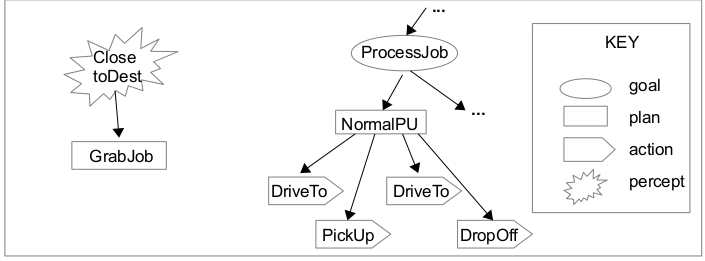
\includegraphics[width=0.75\textwidth]{extending/figures/bdi/fig-taxi-gptree.jpg}
%%}
%\caption{Excerpt of taxi design}
%\label{taxigptree}
%\end{center}
%\end{figure}

\createfigure%
{Excerpt of taxi design}%
{Excerpt of taxi design}%
{\label{taxigptree}}%
{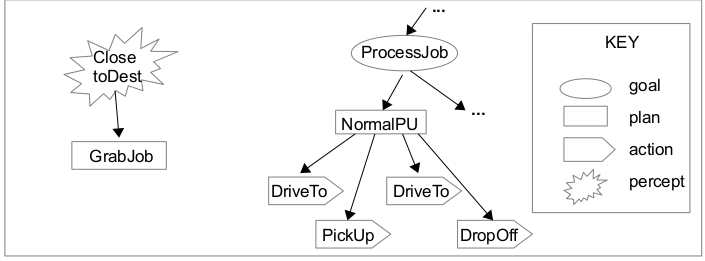
\includegraphics[width=0.75\textwidth]{extending/figures/bdi/fig-taxi-gptree.jpg}}%
{}

% ===========================================================================
\subsection{The \lstinline{ClosetoDest} Percept}
All functions for collecting percepts for the \gls{bdi} system are defined
in the \lstinline{AgentActivityEventHandler} class. Perusal of the existing
functions can ascertain whether the desired percept is already
calculated. For example \lstinline{arriveAtDest} is already defined for use as a
\gls{bdi} percept. 
%
If the percept collection function already exists, all that needs to
happen is to ensure that the agent of the appropriate type is
registered for this percept within the relevant function.
For example, in \lstinline{arriveAtDest()} we have:
\begin{lstlisting}
if agent.type = taxi
   AND agent.loc = dest(agent) \* obtained from infrastructure data *\
       // collect and package this percept
\end{lstlisting}
If we now want this percept provided to agents of type commuter we
must make the first line:
\begin{lstlisting}
if ((agent.type = taxi) OR (agent.type = commuter))
   AND agent.loc = dest(agent) \* obtained from infrastructure data *\
       // collect and package this percept
\end{lstlisting}

The \lstinline{arriveAtDest} function is triggered by the \gls{matsim}
\lstinline{enterLink} event using \gls{matsim} provided callbacks. So
we have defined \lstinline{handleEvent(enterLink)} to call all percept
  collection functions triggered by this event -- in this case
  \lstinline{arriveAtDest}. 

The \lstinline{ClosetoDest} percept will be triggered by the same \gls{matsim}
event \lstinline{enterLink}, so to add this we must add the call to
\lstinline{ClosetoDest} in the \lstinline{handleEvent(enterLink)} and then
  define our \lstinline{ClosetoDest} function within the
  \lstinline{AgentActivityEventHandler} class.  We only want to send the
  \lstinline{ClosetoDest} percept when we first come within the defined
  distance of our destination, not at every step. Therefore the
  \lstinline{ClosetoDest} function must first check whether this percept
  has already been sent to this agent, for the current destination. If
  so, nothing more is done. If not it is ascertained whether the link
  entered is within the desired ``close-to'' distance, and if so the
  percept is registered. For efficiency the first link that
    is ``close-to'' the dest can be calculated and recorded when the
    \lstinline{DriveTo} action is initiated, in which case all that is required is
    to check whether the entered link-ID is the same as the recorded
    ``close-to'' link-ID.

In principle percepts could also be calculated in a function that was
executed after all the agents had been stepped. The important thing is
that when it occurs, the percept is recorded in the percept data
package for that agent. Further work is required to ascertain which
percept collection methods will be most efficient with very large
numbers of agents.

% ===========================================================================
\subsection{The \lstinline{RequestLocation} Query}
Queries are defined in and managed through the \lstinline{MatsimQueryHandler}
class.
A function \lstinline{queryPercept(agent,query,response)} responds to a query by
extracting out the specific query and calling the relevant defined
function. So, for example, in order to respond to the
\lstinline{queryPercept(ownID,``RequestLocation agentID'',loc)} query from an
agent, \lstinline{queryPercept} will contain the code:
\begin{lstlisting}
if percept_type = "RequestLocation"
   loc = getLocation("agentID")
\end{lstlisting}
The \lstinline{getLocation} function will then ascertain the location of
\lstinline{agentID}, storing the value in \lstinline{loc}. 
%
If the query is already defined in \gls{matsim}, nothing further is required
in order to use it in an application.

% ===========================================================================
\subsection{The \lstinline{DriveTo} BDI-Action}
The \lstinline{DriveTo(loc)} \gls{bdi} action is of course the most basic and
commonly used \gls{bdi} action in \gls{matsim}, and is therefore already
implemented in our infrastructure. As long as the appropriate \gls{bdi}
action and parameters are passed in the information package from the
\gls{bdi} system, nothing further is required within \gls{matsim}. However, for
the purpose of illustration, we will assume it has not yet been
implemented, and we will go through the steps of defining a new \gls{bdi}
action with this as an example.

The \lstinline{MATSimActionList} class defines the mappings for all \gls{bdi}
actions in the system and the \gls{matsim} function calls that realize those
\gls{bdi} actions.  Any new \gls{bdi} action must first be added to this list.

The \lstinline{MATSimActionHandler} defines all the functions that
realize the \gls{bdi} actions, as well as a \lstinline{processAction} function
which handles all \gls{bdi} action strings from the \gls{bdi} system,
calling the appropriate helper functions. Thus any new \gls{bdi} action must have
its implementation defined within this class, and must have the appropriate
call to the function added within \lstinline{processAction}.  Let us call
the relevant function that we will add \lstinline{processDriveTo}. This function
will always need the \lstinline{agentID} as a parameter as well as
whatever parameters are provided in the action package. So in our
example we will have the function \lstinline{processDriveTo(agentID, loc)}
which needs to be defined. 
%
The function for the new action must do two key tasks:
\begin{tightenumerate}
\item obtain the \gls{matsim} plan of the relevant agent, and modify it so
  that regular \gls{matsim} execution of the plan will have the desired
  effect.

Generally when the plan is accessed it will have a single dummy
activity with end-time infinity. The end time of this activity must be
set to now, and a leg must be instantiated with the link corresponding
to the destination \lstinline{loc} as the end point, and the links to be
followed as calculated by the router. This leg must then be inserted
into the plan, followed by a new dummy activity instance with end time
infinity. 

\item place the action instance into the list of actions being
  monitored. 
\end{tightenumerate}

It is also necessary to set up recognition of when the action has
finished, so that this information can be sent back to the \gls{bdi} system
and the agent can continue to reason about its next actions.  This is
done via the \gls{matsim} callbacks provided, in the same way as for
detecting percepts. However, the corresponding function, instead of
placing information in the percept package for the agent, will modify
the \lstinline{status} of the relevant \gls{bdi} action instance in the
information package to PASSED, and remove the instance from the list
of actions being monitored. It is also possible to define a condition
under which the action should be considered to have FAILED
and to detect this in a similar way. Alternatively failure can be
managed by sending a percept, and having the \gls{bdi} agent abort the
action as a result\footnote{The simplest way in JACK is to use a
  maintenance condition relying on a belief that is modified as the
  result of a percept.}.

The current structure assumes that multiple actions of a single agent
cannot be executed in parallel (a reasonable assumption for
\gls{matsim}). It is the responsibility of the \gls{bdi} system to only ever have
one \gls{bdi} action per agent active.

Further instructions, as well as examples can be found in our
\gls{bdi}-\gls{matsim} integration repository.

% ===========================================================================
\subsection{Discussion}
An important aspect of the design of a simulation using \gls{bdi} agents
within \gls{matsim} is the decision as to what level of abstraction the \gls{bdi}
actions should be described at. So far we have tended to have \gls{bdi}
actions map to a single \lstinline{leg} or \lstinline{activity} within a
\gls{matsim} plan. However, it is certainly easy to think of \gls{bdi} actions
which combine several such components. Straightforward examples would
be doing grocery shopping, or taking kids to school - both involving a
leg to a destination, an activity at that destination, and a return
leg. There are no immediately obvious advantages associated with \gls{bdi}
actions at higher levels of abstraction (requiring coding of these
actions in \gls{matsim}) vs using lower level \gls{bdi} actions with the higher
level coded as \gls{bdi} plans/goals. Future experience and experimentation
may provide insights that can guide decisions.

% ##################################################################################################################
\section{Examples}
\label{sec:bid-examples}
We describe here two different example uses of \gls{bdi} agents within
\gls{matsim}: a bushfire evacuation simulation, where \gls{matsim} is
being used because traffic flow is a crucial component in bushfire
evacuation, and a taxi application which was developed as a
demonstrator for integration of a \gls{bdi} system with \gls{matsim} \citep{ecai}. We make
some comparison of this approach to incorporating taxis, as compared to
that described in Chapter~\ref{ch:dts} for
incorporating dynamically scheduled vehicles, and with the approaches
to ``within-day replanning'' described in Chapter~\ref{ch:withinday}.

%
Both our example applications use only the \lstinline{Mobsim} engine
(\lstinline{QSim}) of \gls{matsim} and do not do any repeated daily cycles
with plan scoring and modification. There are undoubtedly applications which
could benefit from a combination of \gls{bdi} agents and agents which evolve using
\gls{matsim}'s scoring and replanning, but we have not yet investigated such.

% ===========================================================================
\subsection{Bushfire Example}
The bushfire example (currently) involves modeling of residents and
their decision making behavior about what to do regarding a nearby
bushfire. Potential driving activities include picking up children
from a school or other facility, checking on neighbors or friends,
and driving to a local or further afield destination, possibly via a
specified route. Decision making may involve various factors such as
time of day, beliefs as to what other family members are doing,
warnings and notifications from emergency services, observations of
neighbors, etc. In one approach we have focused on incorporating
well developed and validated actual models of human decision making in
a bushfire situation, developed by a collaborator. Our contribution
has been to integrate this with \gls{matsim}, using our integration
framework, to provide data about any traffic related issues, thus
providing a more valuable simulation to planners. In our other
approach we model both residents, and also an incident
controller. Here our focus has been on technical issues to do with
providing an interactive simulation suitable for use by emergency
services personnel and/or communities for exploration of potential
strategies. 

In the interactive version, the incident controller assigns specified
evacuation centers, and routes, to residents in certain sections of
the town being evacuated. Evacuation of different areas may be started
at different times. Residents follow the instructions of the incident
controller with some probability based on their individual situation
(currently modeled very superficially). Following the suggested route
is achieved by driving via suggested way points  (using the \lstinline{DriveTo} \gls{bdi}
action),  with the \gls{bdi} agent (potentially) re-assessing as each
waypoint is reached. An alternative would be to define a new \gls{bdi}
action \lstinline{DriveToViaWaypoints}. One issue that arose during the
development of this simulation, was that as roads became congested,
\gls{matsim} routing algorithms began developing very circuitous routes,
sometimes going back towards the fire threat. There were two issues
here with regard to developing a realistic simulation: one was that
realistically people would not choose their routes based on global
knowledge of current congestion; the other was that regardless of
congestion people would not head back into the fire zone. The current
solution is to use a routing algorithm which does not take account of
current road speeds, using only static speed limits. Going forward one
may want to assume some knowledge of congestion (based on radio
broadcasts or other social media). A research question is how to best
achieve sharing of responsibility for realistic behavior between
\gls{matsim} and the \gls{bdi} decision making program, with respect to route
selection. 

% ===========================================================================
\subsection{Taxi Example}
The taxi prototype application was developed purely as a proof of
concept which allowed decisions to be made dynamically by the \gls{bdi}
brain on an ongoing basis, then carried out by the \gls{matsim} execution
engine. There is a simple taxi administrator in the \gls{bdi} system, which
generates jobs, posts them to a notice board, and confirms requests
from taxis to take specific jobs. Taxis have plans which allow them to
take jobs from the board, go to a taxi rank or take a break. After
taking a job from the board the taxi drives to the pick-up address,
picks up the passenger, and then drives to the destination and drops
them off. When the taxi is getting close to the destination it looks
on the job board for nearby jobs, and if something suitable is found,
it requests it from the administrator. The only \gls{bdi} action implemented
in this application is a simple \lstinline{DriveTo}. The
\lstinline{ClosetoDest} percept was used as described in Section~\ref{sec:bdi-usage}. 
This application was tested with the Berlin road network
and the 15\,963 agents in the \gls{matsim} sample files, with all agents
operating as \gls{bdi} taxi agents. Profiling showed that by far the
majority of the execution time was spent in route planning, with very
little in the \gls{bdi} reasoning or communication with the \gls{bdi} system.

% ===========================================================================
\subsection{Discussion}
Both evacuation and taxis are discussed in Chapters~\ref{ch:withinday} and~\ref{ch:dts} 
as applications requiring a reactive approach to planning
rather than iteration over many days to find the preferred plan. There
is discussion in Chapter~\ref{ch:dts} of the two implementation options: one
which replaces the \gls{matsim} agent with an agent that considers what to
do at each relevant decision point (particularly intersections); and
the other which leaves the agent code as is, but modifies the agent's
plans when certain events occur. The \gls{bdi} approach has the computational
advantages of the latter, in that only a small subset of the agents
require changes to their plans at any simulation step, and many
existing \gls{matsim} routines can be used to modify the plans. However, it
also has many of the advantages of the former approach in that the
agents are still fully autonomous, in that all decision making occurs
within the \gls{bdi} system. By registering for any percepts which could
potentially cause the agent to change its mind, the agent remains
fully in control at all times. However, it only needs to decide its next action
when it completes the current high level action---which will almost
certainly be orders of magnitude less often than at each intersection---or when 
a percept arrives which indicates a need to reconsider. The
provision of the ability to drop current \gls{bdi} actions (legs or
activities), provides the same level of reactive autonomy as the fully
reactive within day replanning agent, but at what we believe is a
lower computational cost. 
%
Perhaps more importantly than the computational cost savings is the
fact that the agent decision making can be programmed in a framework
that is at a high level of abstraction, using goals, plans and
beliefs, within existing highly efficient platforms such as JACK
\citep{jackref}, Jadex \citep{jadex2005} or Jason \citep{jason}. Design
tools for developing such agents also already exist
\citep{prometheusbook}. One study has shown that using a \gls{bdi} language
makes program development hugely more efficient than programming in
\gls{java} \citep{benfield}. The close mapping between intuitively
understandable design diagrams, and the program code which implements
this in a \gls{bdi} system, is also highly advantageous for validating
design of realistic agents with domain experts. We have discussed
design of resident agents in a sandbagging flood scenario, with
emergency services personnel having a deep understanding of the
domain, and found the representation to be effective. We consider that
this representational aspect can be a significant advantage when
compared to programming the agent using the \lstinline{DynAgentLogic}
facility described in Chapter~\ref{ch:dts}.
%\label{ch:dts} 13
%\label{ch:withinday}7

% ##################################################################################################################








